\documentclass{article}
\usepackage{graphicx} % Required for inserting images
\usepackage{amsmath}
\usepackage{enumitem}
\usepackage[paper=a4paper, margin=2cm]{geometry}
\usepackage{eurosym}
\usepackage{xcolor}
\usepackage{float}
\usepackage{pgfplots}
\usepackage[plain, onelanguage]{algorithm2e}

\title{Algorithmic Methods for Mathematical Models\\
  Course Project }
\author{Tim Wichelmann\\ \texttt{tim.wichelmann@estudiantat.upc.edu}\\[1ex] % [1ex] adds vertical space
  Jakob Eberhardt\\ \texttt{jakob.eberhardt@estudiantat.upc.edu}}
\date{\today}
\pgfplotsset{compat=1.18} 
\begin{document}

\maketitle
\thispagestyle{empty}
\newpage
\setcounter{page}{1}
\tableofcontents
% \lstlistoflistings
\listoffigures
\newpage

\section{Formal Problem Statement}
\subsection*{Given}

We have as inputs the following variables:
\begin{itemize}
    \item $profit_i$ : Profit associated with order $i$ in \euro{}.
    \item $length_i$ : Required number of time slots to process order $i$.
    \item $min\_deliver_i$ : First time slot in which order $i$ can be picked up by the customer.
    \item $max\_deliver_i$ : Last time slot order $i$ can be picked up by the customer.
    \item $surface_i$ : Oven surface required to bake order $i$ in $m^2$.
    \item $surface\_capacity$ : Oven surface available in the bakery in $m^2$.
\end{itemize}
If an order is processed, is has to be picked up in the same time slot in which it will be finished.
Due to the limited surface capacity, the  oven surface occupied by the scheduled orders can never exceed $surface\_capacity$ for any given time slot.

At any time, the total surface of the bread that is being baked cannot exceed this capacity.
\subsection*{Auxiliary Indices} %% sind meiner Ansicht nach auch ganz normal Teil des Inputs und auch nicht wirklich Indizes
\begin{itemize}
    \item $n$ : The number of unattended orders which can be picked for the next period.
    \item $t$ : The number of available time slots in the next period.
\end{itemize}

\subsection*{Output}
The output consists of a matrix of size $n \times t$.
It represents a timetable indicating if and when an order should be processed. 

\subsection*{Objective}
Maximize the profit for the planned period.

\section{Integer Linear Programming Model}

\subsection{Decision variables}
\begin{itemize}
    \item $y$ is a matrix of size $n \times t$ consisting of binary variables which indicates if the order $i$ will be baked in time slot $j$.
\end{itemize}

\subsection{Auxiliary variables}

\begin{itemize}
\item $x_i$ is a binary variable indicating whether order $i$ has the right amount of time slots assigned to it. 
We use it as an indicator of 
% \item $\mathit{start}_{ij}$ denotes the time slot $j$ in which the baking process of order $i$ is started.
\item $\mathit{start}_{i}$ denotes the time slot in which the baking process of order $i$ is started.
\item $\mathit{end}_{i}$ denotes the time slot in which the baking process of order $i$ will be finished.
\end{itemize}

\subsection{Objective function}

\begin{equation*}
  \max \sum^n_{i = 1} \mathit{profit}_i \: x_i
\end{equation*}

\subsection{Constraints}

Subject to

\begin{itemize}
 %    \item Every processed order has finished baking before the maximum delivery time: 
 %    \begin{equation}
 %    \mathit{start}_{ij}(j + \mathit{length}_i - 1) \leq \mathit{max\_deliver}_i, (1 \leq i \leq n, 1 \leq j \leq t)
 %    \end{equation}
 %    \item Every processed order has finished baking after the minimum delivery time:
 %    \begin{equation}
 %        j + \mathit{length}_i - 1 \geq \mathit{start}_{ij} \: \mathit{min\_deliver}_i, (1 \leq i \leq n, 1 \leq j \leq t) 
 %    \end{equation}
    \item In every time slot, the space capacity is respected:
    
    \begin{align}
        \sum^n_{i=1}\mathit{surface}_i \: y_{ij} &\leq \mathit{surface\_capacity}, &&(1 \leq j \leq t)
    \end{align}
    
 %    % \item The auxiliary variable $\mathit{start}_i$ has the intended meaning:
 %    % \begin{equation}
 %    %     \mathit{start}_i \leq \mathit{max\_deliver}_i - \mathit{length}_i
 %    % \end{equation}
    % \item We assign the correct amount of time slots or zero time slots to every order:
    % \begin{equation}
    %     \sum^t_{j = 1} y_{ij} = x_i \: \mathit{length}_i, (1 \leq i \leq n)
    % \end{equation}
 %    \item The time slots assigned to this order are contiguous (If an order $i$ starts in time slot $j$, it occupies the consecutive time slots from $j$ to $j + length_i$:
 % %%   \begin{equation}
 % %%       \mathit{start}_{ij} = 1 \doublearrow \sum^{j+\mathit{length}_i-1}_{k=j} y_{i,k} = \mathit{length}_i 
 % %%   \end{equation}
 %        \begin{equation}
 %        \sum^{j+\mathit{length}_i-1}_{k=j} y_{i,k} \geq \mathit{start_}{ij} \mathit{length}_i, (1 \leq i \leq n, 1 \leq j \leq t - \mathit{length}_i + 1 )
 %    \end{equation}
 %    \item Each order only has one start point:
 %    \begin{equation}
 %    \sum^{t}_{j = 1} \mathit{start}_{ij} = x_i, (1 \leq i \leq n)
 %    \end{equation}

    \item Each order is started in a time slot which allows it to finish in the delivery window:
    \begin{align}
    \mathit{start}_i &\leq \mathit{max\_start}_i, \\
    \mathit{min\_start}_i &\leq \mathit{start}_i, &&(1 \leq i \leq n)	
    \end{align}
    
    \item If an order $i$ is part of the schedule, it is assigned the $\mathit{length}_i - 1$ contiguous time slots from $\mathit{start}_i$ to $\mathit{end}_i$:
    \begin{align}
      j &\geq \mathit{start}_i - (t+1) * (1-\mathit{geq\_start}_{ij}) \\
      \mathit{start}_i &\geq j - (t+1) * \mathit{geq\_start}_{ij} \\
      \mathit{end}_i &\geq j - (t+1) * (1-\mathit{leq\_end}_{ij}) \\
      j &\geq \mathit{end}_i - (t+1) * \mathit{leq\_end}_{ij} \\
      0 &\leq \mathit{geq\_start}_{ij} + \mathit{leq\_end}_{ij} - 2 * y_{ij}, &&(1 \leq i \leq n, \mathit{min\_start}_i \leq j \leq \mathit{max\_deliver}_i) 
   \end{align}

    \item If an order $i$ is part of the schedule, its end time $\mathit{end}_i$ is equal to $\mathit{start}_i + \mathit{length}_i - 1$. 
      If order $i$ is not part of the schedule, this is indicated by the fact that $\mathit{start}_i > \mathit{end}_i$.
    \begin{align}
        \mathit{end}_i &= \mathit{start}_i + x_i \: \mathit{length}_i - 1, &&(1 \leq i \leq n)
    \end{align}

     \item %The following constraints are not necessary to obtain a correct solution.
     % But they improve the performance of the solver by eliminating infeasible solutions early on.
     % The first of these constraints is: 
     If an order is part of the schedule, we assign the correct amount of time slots to it.
     Otherwise we assign zero time slots to it:    
    \begin{align}
        \sum^{\mathit{max\_deliver}_i}_{j = \mathit{min\_start}_i} y_{ij} &= x_i \: \mathit{length}_i, &&(1 \leq i \leq n)
    \end{align}
    
    \item There are no orders assigned to time slots which are infeasible for this order because of the delivery window:    
    \begin{align}
     \sum_{j = 1}^{\mathit{min\_start}_i-1} y_{ij} &= 0, &&(1 \leq i \leq n) \\
   \sum_{j = \mathit{max\_deliver}_i+1}^t y_{ij} &= 0, &&(1 \leq i \leq n) 
    \end{align}
\end{itemize}

\section{Meta-heuristics}
\subsection{Greedy constructive}
\begin{center}
\begin{algorithm}[H]
\KwIn{orders}
solution $\gets \emptyset$ \\
sortedOrders $\gets$ sort(orders, $\lambda \: x$ : orderRating($x$), DESC) \\
\ForEach{order in sortedOrders}{
    candidateSlots $\gets$ findFeasibleAssignments(order, solution)\\
    \If{$|candidateSlots| = 0$} {continue with next iteration}
    sortedCandidates $\gets$ sort(candidateSlots, $\lambda \: x$ : slotRating($x$, solution), DESC) \\
    candidate $\gets$ sortedCandidates[0]\\
    assign(order, startTime(candidate), solution)\\
}
\Return{solution}\;
\end{algorithm}
\end{center}

\subsection{Local search}
\begin{center}
\begin{algorithm}[H]
    \KwIn{Solution S} 
    iteration $\gets$ 0\\
    \While{time $<$ maxTime}{
        oldOrders $\gets$ sort(attendedOrders(S), $\lambda \: x$ : eassignmentRating(x), DESC)\\
        oldOrder $\gets$ oldOrders[mod(iteration, length(oldOrders))]\\
        
        currentProfit $\gets$ fitness(S)\\

        newOrders $\gets$  sort(unattendedOrders(S), $\lambda \: x$ : profti(x), DESC)\\

        oldStart $\gets$ startsAt(S, oldOrderId)\\
        unassign(S, oldOrderId)\\

        \ForEach{newOrder in newOrders}{
            assignments $\gets$  findFeasibleAssignments(S, newOrder)\\
            \If{$|$assignments$| = 0$}{
                continue with next iteration\\
            }
            move $\gets$ (oldOrder, newOrder, start(assignments[0]))\\
            neighborHighestProfit $\gets$ evaluateNeighbor(S, move)\\

            \If{currentProfit $<$ neighborHighestProfit}{
                neighbor $\gets$ createNeighborSolution(solution, move)\\
                \lIf{neighbor = NULL}{continue with next iteration}
            }
        }
        \eIf{neighbor = NULL}{
            solution.assign(oldOrderId, oldStart) \\
            iteration $\gets$ iteration + 1 \\
            continue with next iteration\\
            }
            {
                neighborFitness $\gets$ getFitness(neighbor)\\
                incumbent $\gets$ neighbor \\
                incumbentFitness $\gets$ neighborFitness \\
                iteration $\gets$ 0\\
            }
            }
    \Return{incumbent}
\end{algorithm}
\end{center}

\subsection{GRASP}
\begin{center}
\begin{algorithm}[H]
GRASP constructive phase \\
Initialize C \\
S $\gets$ $\emptyset$ \\
\While{S is not a solution}{ \\
Evaluate q(c) for all c $\in$ C \\
q^{min} $\gets min \{q(c) | c \in C\}$ \\
q^{max} $\gets max \{q(c) | c \in C\}$ \\
RCL_{max} $\gets \{c \in C | q(c) \geq q^{max} - \alpha(q^{max} - q^{min})\}$ \\
Select c $\in$ RCL at random \\
S $\gets$ S $\cup$ {c} \\
update C \\
}
\Return{S} \\
\end{algorithm}
\end{center}

\section{Parameter Tuning}

\section{Comparison}
%%% Optimal 125, 125_plot.dat, laufzeit: 3h
\begin{figure}[H]
\centering
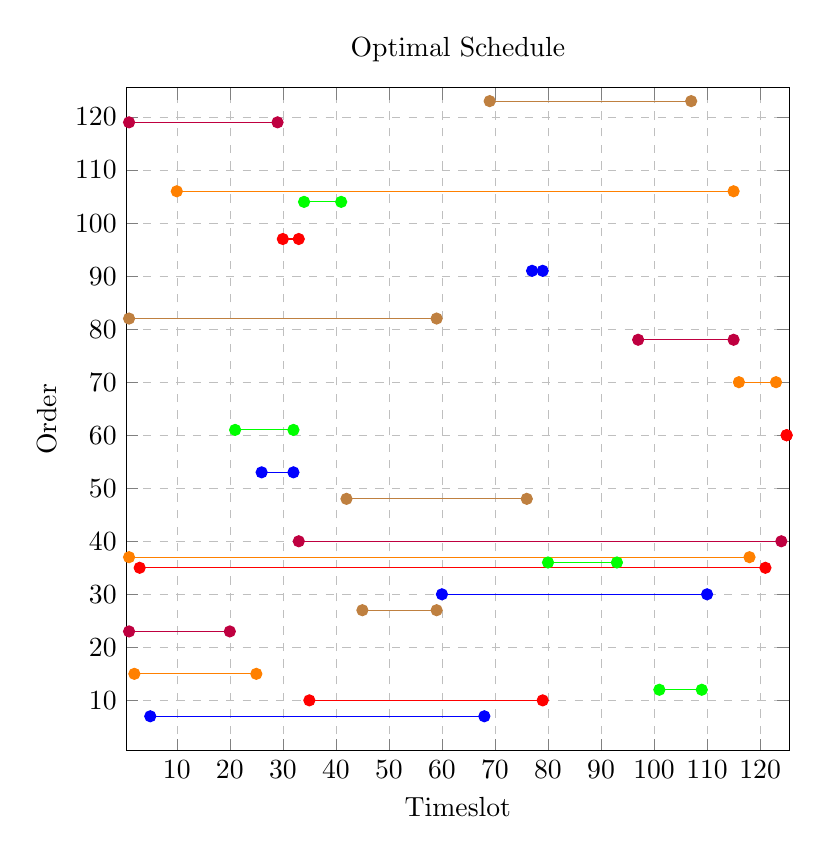
\begin{tikzpicture}
\begin{axis}[
    title={Optimal Schedule},
    xlabel={Timeslot},
    ylabel={Order},
    xmin=0.5, xmax=125.5, 
    ymin=0.5, ymax=125.5, 
    xtick={10,20,30,40,50,60,70,80,90,100, 110, 120},
    ytick={10,20,30,40,50,60,70,80,90,100, 110, 120},
    grid=both,
    grid style={line width=.1pt, draw=gray!10},
    major grid style={line width=.2pt, draw=gray!50},
    legend pos=north east,
    ymajorgrids=true,
    xmajorgrids=true,
    grid style=dashed,
    width=10cm,
    height=10cm,
]
\addplot[color=blue, mark=*] coordinates {(5, 7) (68, 7)};
\addplot[color=red, mark=*] coordinates {(35, 10) (79, 10)};
\addplot[color=green, mark=*] coordinates {(101, 12) (109, 12)};
\addplot[color=orange, mark=*] coordinates {(2, 15) (25, 15)};
\addplot[color=purple, mark=*] coordinates {(1, 23) (20, 23)};
\addplot[color=brown, mark=*] coordinates {(45, 27) (59, 27)};
\addplot[color=blue, mark=*] coordinates {(60, 30) (110, 30)};
\addplot[color=red, mark=*] coordinates {(3, 35) (121, 35)};
\addplot[color=green, mark=*] coordinates {(80, 36) (93, 36)};
\addplot[color=orange, mark=*] coordinates {(1, 37) (118, 37)};
\addplot[color=purple, mark=*] coordinates {(33, 40) (124, 40)};
\addplot[color=brown, mark=*] coordinates {(42, 48) (76, 48)};
\addplot[color=blue, mark=*] coordinates {(26, 53) (32, 53)};
\addplot[color=red, mark=*] coordinates {(125, 60) (125, 60)};
\addplot[color=green, mark=*] coordinates {(21, 61) (32, 61)};
\addplot[color=orange, mark=*] coordinates {(116, 70) (123, 70)};
\addplot[color=purple, mark=*] coordinates {(97, 78) (115, 78)};
\addplot[color=brown, mark=*] coordinates {(1, 82) (59, 82)};
\addplot[color=blue, mark=*] coordinates {(77, 91) (79, 91)};
\addplot[color=red, mark=*] coordinates {(30, 97) (33, 97)};
\addplot[color=green, mark=*] coordinates {(34, 104) (41, 104)};
\addplot[color=orange, mark=*] coordinates {(10, 106) (115, 106)};
\addplot[color=purple, mark=*] coordinates {(1, 119) (29, 119)};
\addplot[color=brown, mark=*] coordinates {(69, 123) (107, 123)};

\end{axis}
\end{tikzpicture}
\caption[Example of an Optimal Schedule]{This schedule represents a optimal solution for a given data set of 125 orders and 125 time slots. The profit of this optimal solution is 164 \euro{}.}
\label{fig:extended_schedule_opt}
\end{figure}

%%% 125 Heuristik, 125_plot.dat, getAddedValue : profit only
\begin{figure}[H]
\centering
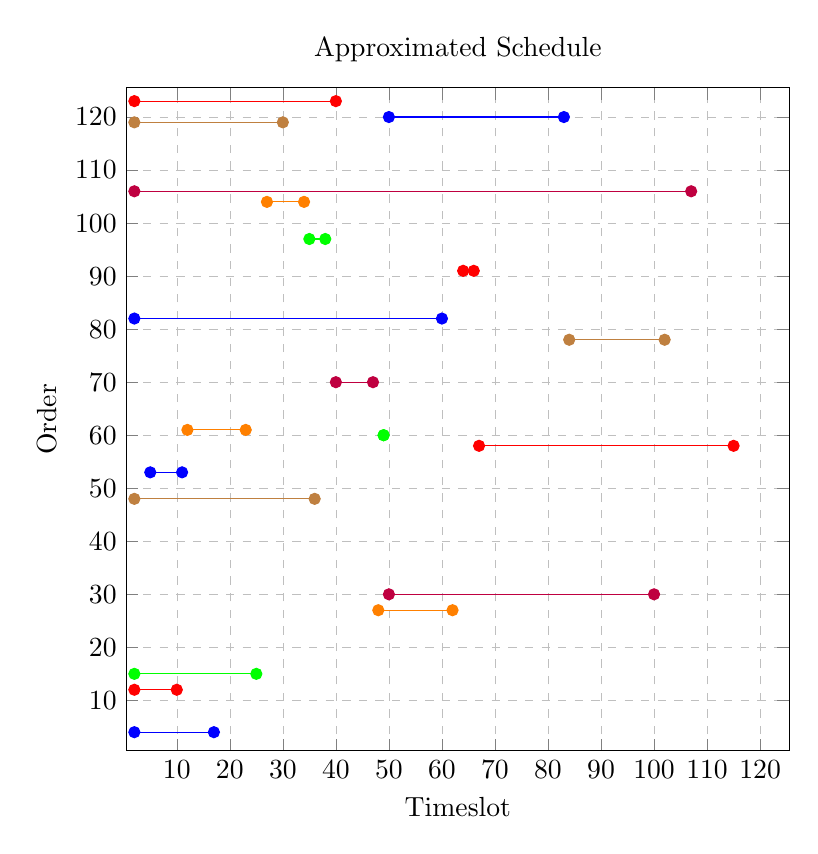
\begin{tikzpicture}
\begin{axis}[
    title={Approximated Schedule},
    xlabel={Timeslot},
    ylabel={Order},
    xmin=0.5, xmax=125.5, 
    ymin=0.5, ymax=125.5, 
    xtick={10,20,30,40,50,60,70,80,90,100, 110, 120},
    ytick={10,20,30,40,50,60,70,80,90,100, 110, 120},
    grid=both,
    grid style={line width=.1pt, draw=gray!10},
    major grid style={line width=.2pt, draw=gray!50},
    legend pos=north east,
    ymajorgrids=true,
    xmajorgrids=true,
    grid style=dashed,
    width=10cm,
    height=10cm,
]
\addplot[color=blue, mark=*] coordinates {(2, 4) (17, 4)};
\addplot[color=red, mark=*] coordinates {(2, 12) (10, 12)};
\addplot[color=green, mark=*] coordinates {(2, 15) (25, 15)};
\addplot[color=orange, mark=*] coordinates {(48, 27) (62, 27)};
\addplot[color=purple, mark=*] coordinates {(50, 30) (100, 30)};
\addplot[color=brown, mark=*] coordinates {(2, 48) (36, 48)};
\addplot[color=blue, mark=*] coordinates {(5, 53) (11, 53)};
\addplot[color=red, mark=*] coordinates {(67, 58) (115, 58)};
\addplot[color=green, mark=*] coordinates {(49, 60) (49, 60)};
\addplot[color=orange, mark=*] coordinates {(12, 61) (23, 61)};
\addplot[color=purple, mark=*] coordinates {(40, 70) (47, 70)};
\addplot[color=brown, mark=*] coordinates {(84, 78) (102, 78)};
\addplot[color=blue, mark=*] coordinates {(2, 82) (60, 82)};
\addplot[color=red, mark=*] coordinates {(64, 91) (66, 91)};
\addplot[color=green, mark=*] coordinates {(35, 97) (38, 97)};
\addplot[color=orange, mark=*] coordinates {(27, 104) (34, 104)};
\addplot[color=purple, mark=*] coordinates {(2, 106) (107, 106)};
\addplot[color=brown, mark=*] coordinates {(2, 119) (30, 119)};
\addplot[color=blue, mark=*] coordinates {(50, 120) (83, 120)};
\addplot[color=red, mark=*] coordinates {(2, 123) (40, 123)};
\end{axis}
\end{tikzpicture}
\caption[Example of an Approximated Schedule]{This schedule was created for 125 possible orders, resulting in an optimized profit of 126 \euro{}. The greedy algorithm was tuned towards preferring orders with high profit.}
\label{fig:125_schedule_approx}
\end{figure}

%%% 125 GRASP, 125_plot.dat, random assignments a=1, t=120
\begin{figure}[H]
\centering
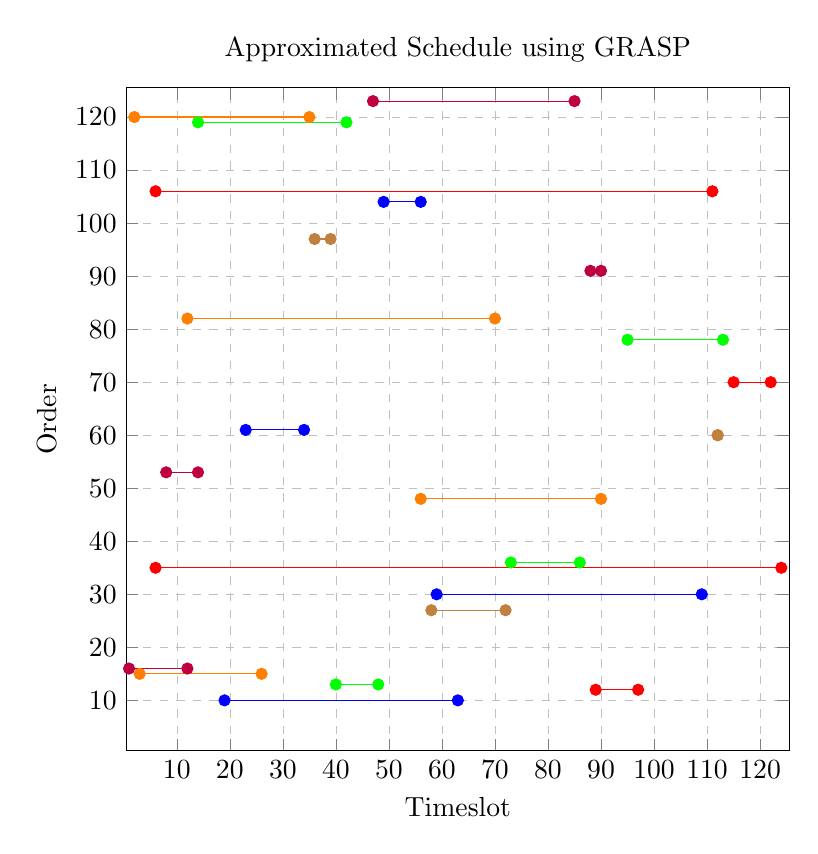
\begin{tikzpicture}
\begin{axis}[
    title={Approximated Schedule using GRASP},
    xlabel={Timeslot},
    ylabel={Order},
    xmin=0.5, xmax=125.5, 
    ymin=0.5, ymax=125.5, 
    xtick={10,20,30,40,50,60,70,80,90,100, 110, 120},
    ytick={10,20,30,40,50,60,70,80,90,100, 110, 120},
    grid=both,
    grid style={line width=.1pt, draw=gray!10},
    major grid style={line width=.2pt, draw=gray!50},
    legend pos=north east,
    ymajorgrids=true,
    xmajorgrids=true,
    grid style=dashed,
    width=10cm,
    height=10cm,
]
\addplot[color=blue, mark=*] coordinates {(19, 10) (63, 10)};
\addplot[color=red, mark=*] coordinates {(89, 12) (97, 12)};
\addplot[color=green, mark=*] coordinates {(40, 13) (48, 13)};
\addplot[color=orange, mark=*] coordinates {(3, 15) (26, 15)};
\addplot[color=purple, mark=*] coordinates {(1, 16) (12, 16)};
\addplot[color=brown, mark=*] coordinates {(58, 27) (72, 27)};
\addplot[color=blue, mark=*] coordinates {(59, 30) (109, 30)};
\addplot[color=red, mark=*] coordinates {(6, 35) (124, 35)};
\addplot[color=green, mark=*] coordinates {(73, 36) (86, 36)};
\addplot[color=orange, mark=*] coordinates {(56, 48) (90, 48)};
\addplot[color=purple, mark=*] coordinates {(8, 53) (14, 53)};
\addplot[color=brown, mark=*] coordinates {(112, 60) (112, 60)};
\addplot[color=blue, mark=*] coordinates {(23, 61) (34, 61)};
\addplot[color=red, mark=*] coordinates {(115, 70) (122, 70)};
\addplot[color=green, mark=*] coordinates {(95, 78) (113, 78)};
\addplot[color=orange, mark=*] coordinates {(12, 82) (70, 82)};
\addplot[color=purple, mark=*] coordinates {(88, 91) (90, 91)};
\addplot[color=brown, mark=*] coordinates {(36, 97) (39, 97)};
\addplot[color=blue, mark=*] coordinates {(49, 104) (56, 104)};
\addplot[color=red, mark=*] coordinates {(6, 106) (111, 106)};
\addplot[color=green, mark=*] coordinates {(14, 119) (42, 119)};
\addplot[color=orange, mark=*] coordinates {(2, 120) (35, 120)};
\addplot[color=purple, mark=*] coordinates {(47, 123) (85, 123)};

\end{axis}
\end{tikzpicture}
\caption[Example of an Approximated Schedule]{This schedule was created for 125 possible orders using the GRASP solver, resulting in an optimized profit of 146 \euro{}.}
\label{fig:125_schedule_approx}
\end{figure}

%%% Optimal 100, 100.dat, laufzeit: 15min
\begin{figure}[H]
\centering
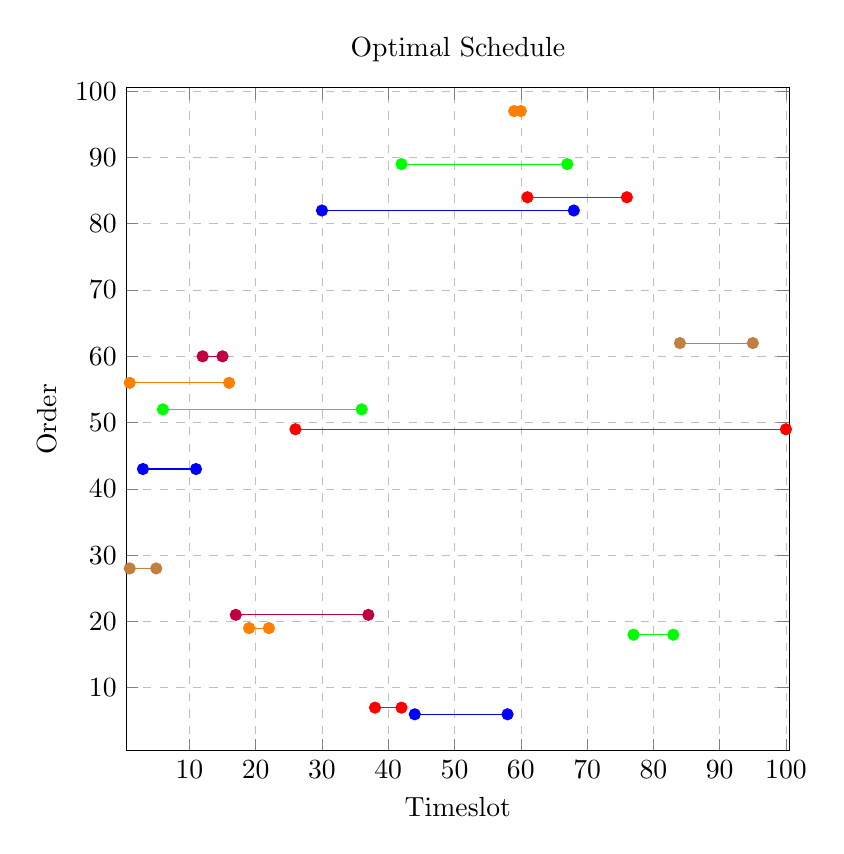
\begin{tikzpicture}
\begin{axis}[
    title={Optimal Schedule},
    xlabel={Timeslot},
    ylabel={Order},
    xmin=0.5, xmax=100.5, 
    ymin=0.5, ymax=100.5, 
    xtick={10,20,30,40,50,60,70,80,90,100},
    ytick={10,20,30,40,50,60,70,80,90,100},
    grid=both,
    grid style={line width=.1pt, draw=gray!10},
    major grid style={line width=.2pt, draw=gray!50},
    legend pos=north east,
    ymajorgrids=true,
    xmajorgrids=true,
    grid style=dashed,
    width=10cm,
    height=10cm,
]
\addplot[color=blue, mark=*] coordinates {(44, 6) (58, 6)};
\addplot[color=red, mark=*] coordinates {(38, 7) (42, 7)};
\addplot[color=green, mark=*] coordinates {(77, 18) (83, 18)};
\addplot[color=orange, mark=*] coordinates {(19, 19) (22, 19)};
\addplot[color=purple, mark=*] coordinates {(17, 21) (37, 21)};
\addplot[color=brown, mark=*] coordinates {(1, 28) (5, 28)};
\addplot[color=blue, mark=*] coordinates {(3, 43) (11, 43)};
\addplot[color=red, mark=*] coordinates {(26, 49) (100, 49)};
\addplot[color=green, mark=*] coordinates {(6, 52) (36, 52)};
\addplot[color=orange, mark=*] coordinates {(1, 56) (16, 56)};
\addplot[color=purple, mark=*] coordinates {(12, 60) (15, 60)};
\addplot[color=brown, mark=*] coordinates {(84, 62) (95, 62)};
\addplot[color=blue, mark=*] coordinates {(30, 82) (68, 82)};
\addplot[color=red, mark=*] coordinates {(61, 84) (76, 84)};
\addplot[color=green, mark=*] coordinates {(42, 89) (67, 89)};
\addplot[color=orange, mark=*] coordinates {(59, 97) (60, 97)};

\end{axis}
\end{tikzpicture}
\caption[Example of an Optimal Schedule]{This schedule represents a optimal solution for a given data set of 100 orders and 100 time slots. The profit of this optimal solution is 93 \euro{}.}
\label{fig:extended_schedule_opt}
\end{figure}

%%% 100 Heuristik, 100_plot.dat, getAddedValue : profit only
\begin{figure}[H]
\centering
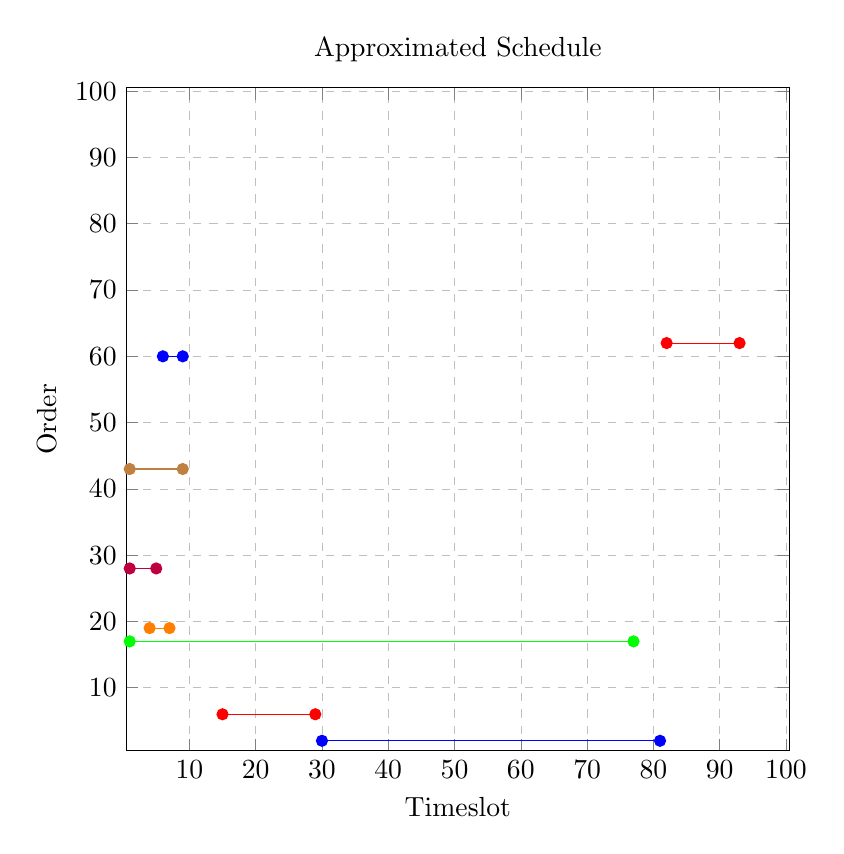
\begin{tikzpicture}
\begin{axis}[
    title={Approximated Schedule},
    xlabel={Timeslot},
    ylabel={Order},
    xmin=0.5, xmax=100.5, 
    ymin=0.5, ymax=100.5, 
    xtick={10,20,30,40,50,60,70,80,90,100},
    ytick={10,20,30,40,50,60,70,80,90,100},
    grid=both,
    grid style={line width=.1pt, draw=gray!10},
    major grid style={line width=.2pt, draw=gray!50},
    legend pos=north east,
    ymajorgrids=true,
    xmajorgrids=true,
    grid style=dashed,
    width=10cm,
    height=10cm,
]
\addplot[color=blue, mark=*] coordinates {(30, 2) (81, 2)};
\addplot[color=red, mark=*] coordinates {(15, 6) (29, 6)};
\addplot[color=green, mark=*] coordinates {(1, 17) (77, 17)};
\addplot[color=orange, mark=*] coordinates {(4, 19) (7, 19)};
\addplot[color=purple, mark=*] coordinates {(1, 28) (5, 28)};
\addplot[color=brown, mark=*] coordinates {(1, 43) (9, 43)};
\addplot[color=blue, mark=*] coordinates {(6, 60) (9, 60)};
\addplot[color=red, mark=*] coordinates {(82, 62) (93, 62)};

\end{axis}
\end{tikzpicture}
\caption[Example of an Approximated Schedule]{This schedule was created for 100 possible orders, resulting in an optimized profit of 51 \euro{}. The greedy algorithm was tuned towards preferring orders with high profit.}
\label{fig:extended_schedule_approx}
\end{figure}

% \begin{figure}[H]
% \centering
% \begin{tikzpicture}
% \begin{axis}[
%     title={Approximated Schedule Visualization},
%     xlabel={Timeslot},
%     ylabel={Order},
%     xmin=0.5, xmax=75.5, 
%     ymin=0.5, ymax=75.5, 
%     xtick={5,10,15,20,25,30,35,40,45,50,55,60,65,70,75},
%     ytick={1,5,10,15,20,25,30,35,40,45,50,55,60,65,70,75},
%     grid=both,
%     grid style={line width=.1pt, draw=gray!10},
%     major grid style={line width=.2pt, draw=gray!50},
%     legend pos=north east,
%     ymajorgrids=true,
%     xmajorgrids=true,
%     grid style=dashed,
% ]
% \addplot[color=blue, mark=*] coordinates {(50, 4) (51, 4)};
% \addplot[color=red, mark=*] coordinates {(25, 12) (27, 12)};
% \addplot[color=green, mark=*] coordinates {(62, 14) (62, 14)};
% \addplot[color=orange, mark=*] coordinates {(52, 24) (61, 24)};
% \addplot[color=purple, mark=*] coordinates {(33, 38) (49, 38)};
% \addplot[color=brown, mark=*] coordinates {(23, 40) (27, 40)};
% \addplot[color=blue, mark=*] coordinates {(29, 43) (32, 43)};
% \addplot[color=red, mark=*] coordinates {(1, 48) (34, 48)};
% \addplot[color=green, mark=*] coordinates {(1, 58) (20, 58)};
% \addplot[color=orange, mark=*] coordinates {(6, 59) (74, 59)};
% \addplot[color=purple, mark=*] coordinates {(3, 61) (23, 61)};
% \addplot[color=brown, mark=*] coordinates {(28, 63) (28, 63)};
% \addplot[color=blue, mark=*] coordinates {(1, 64) (27, 64)};
% \addplot[color=red, mark=*] coordinates {(37, 66) (49, 66)};
% \addplot[color=green, mark=*] coordinates {(27, 69) (27, 69)};
% \end{axis}
% \end{tikzpicture}
% \caption[Example of an Optimal Solution]{Optimal with value 102.}
% \label{fig:compact_schedule_opt}
% \end{figure}

% \begin{figure}[H]
% \centering
% \begin{tikzpicture}
% \begin{axis}[
%     title={Approximated Schedule Visualization},
%     xlabel={Timeslot},
%     ylabel={Order},
%     xmin=0.5, xmax=75.5, 
%     ymin=0.5, ymax=75.5, 
%     xtick={5,10,15,20,25,30,35,40,45,50,55,60,65,70,75},
%     ytick={1,5,10,15,20,25,30,35,40,45,50,55,60,65,70,75},
%     grid=both,
%     grid style={line width=.1pt, draw=gray!10},
%     major grid style={line width=.2pt, draw=gray!50},
%     legend pos=north east,
%     ymajorgrids=true,
%     xmajorgrids=true,
%     grid style=dashed,
% ]
% \addplot[color=blue, mark=*] coordinates {(46, 1) (58, 1)};
% \addplot[color=red, mark=*] coordinates {(44, 4) (45, 4)};
% \addplot[color=green, mark=*] coordinates {(16, 12) (18, 12)};
% \addplot[color=orange, mark=*] coordinates {(19, 14) (19, 14)};
% \addplot[color=purple, mark=*] coordinates {(1, 18) (7, 18)};
% \addplot[color=brown, mark=*] coordinates {(25, 24) (34, 24)};
% \addplot[color=blue, mark=*] coordinates {(12, 40) (16, 40)};
% \addplot[color=red, mark=*] coordinates {(21, 43) (24, 43)};
% \addplot[color=green, mark=*] coordinates {(1, 48) (34, 48)};
% \addplot[color=orange, mark=*] coordinates {(2, 62) (10, 62)};
% \addplot[color=purple, mark=*] coordinates {(20, 63) (20, 63)};
% \addplot[color=brown, mark=*] coordinates {(35, 64) (61, 64)};
% \addplot[color=blue, mark=*] coordinates {(17, 69) (17, 69)};
% \end{axis}
% \end{tikzpicture}
% \caption[Example of an Approximated Schedule]{This schedule was created using the plain greedy implementation to handle 75 orders. It results in a profit of 65.}
% \label{fig:compact_schedule_approx}
% \end{figure}


\section{Summary}

\end{document}
